\documentclass{extbook}[14pt]
\usepackage{multicol, enumerate, enumitem, hyperref, color, soul, setspace, parskip, fancyhdr, amssymb, amsthm, amsmath, bbm, latexsym, units, mathtools}
\everymath{\displaystyle}
\usepackage[headsep=0.5cm,headheight=0cm, left=1 in,right= 1 in,top= 1 in,bottom= 1 in]{geometry}
\usepackage{dashrule}  % Package to use the command below to create lines between items
\newcommand{\litem}[1]{\item #1

\rule{\textwidth}{0.4pt}}
\pagestyle{fancy}
\lhead{}
\chead{Answer Key for Progress Quiz 4 Version B}
\rhead{}
\lfoot{6286-1986}
\cfoot{}
\rfoot{Fall 2020}
\begin{document}
\textbf{This key should allow you to understand why you choose the option you did (beyond just getting a question right or wrong). \href{https://xronos.clas.ufl.edu/mac1105spring2020/courseDescriptionAndMisc/Exams/LearningFromResults}{More instructions on how to use this key can be found here}.}

\textbf{If you have a suggestion to make the keys better, \href{https://forms.gle/CZkbZmPbC9XALEE88}{please fill out the short survey here}.}

\textit{Note: This key is auto-generated and may contain issues and/or errors. The keys are reviewed after each exam to ensure grading is done accurately. If there are issues (like duplicate options), they are noted in the offline gradebook. The keys are a work-in-progress to give students as many resources to improve as possible.}

\rule{\textwidth}{0.4pt}

\begin{enumerate}\litem{
Choose the graph of the equation below.
\[ f(x) = \frac{1}{x - 1} + 3 \]
The solution is the graph below, which is option A.
\begin{center}
    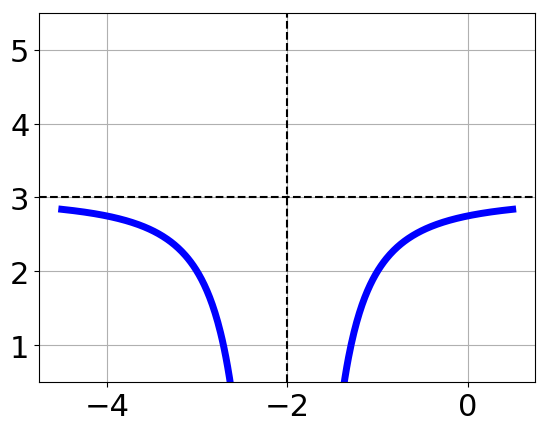
\includegraphics[width=0.3\textwidth]{../Figures/rationalEquationToGraphAB.png}
\end{center}\begin{enumerate}[label=\Alph*.]
\begin{multicols}{2}
\item 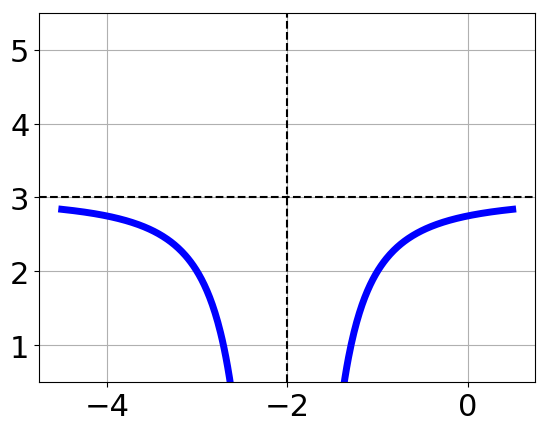
\includegraphics[width = 0.3\textwidth]{../Figures/rationalEquationToGraphAB.png}
\item 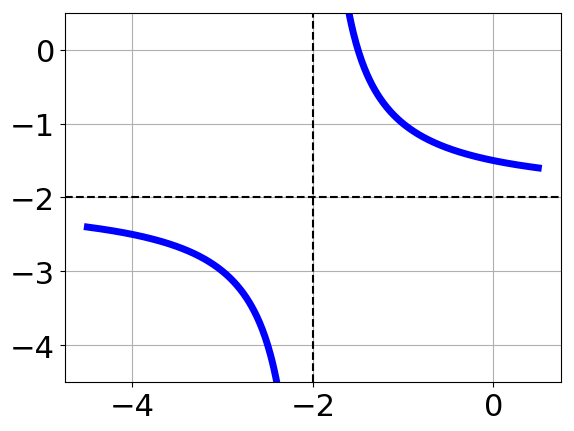
\includegraphics[width = 0.3\textwidth]{../Figures/rationalEquationToGraphBB.png}
\item 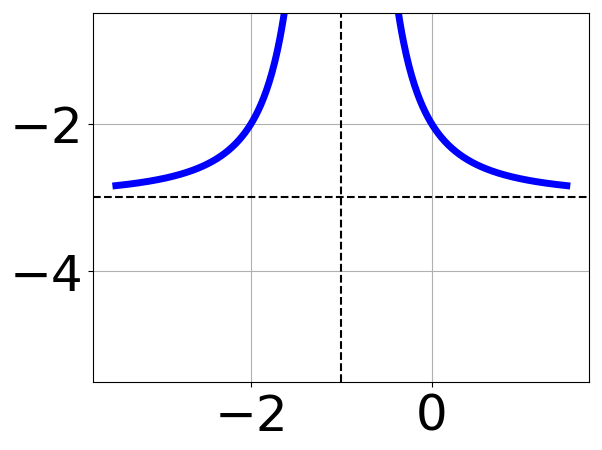
\includegraphics[width = 0.3\textwidth]{../Figures/rationalEquationToGraphCB.png}
\item 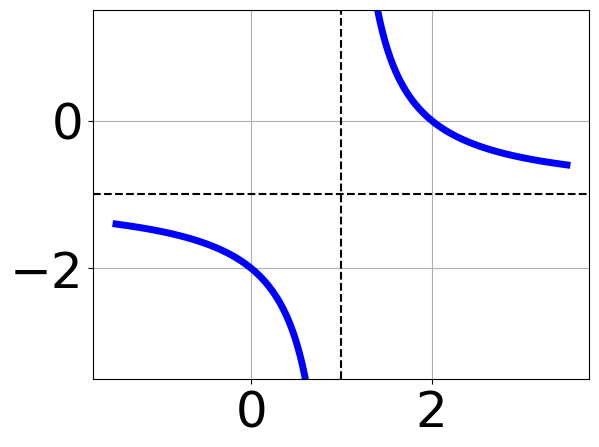
\includegraphics[width = 0.3\textwidth]{../Figures/rationalEquationToGraphDB.png}
\end{multicols}\item None of the above.\end{enumerate}
\textbf{General Comment:} Remember that the general form of a basic rational equation is $ f(x) = \frac{a}{(x-h)^n} + k$, where $a$ is the leading coefficient (and in this case, we assume is either $1$ or $-1$), $n$ is the degree (in this case, either $1$ or $2$), and $(h, k)$ is the intersection of the asymptotes.
}
\litem{
Choose the equation of the function graphed below.

\begin{center}
    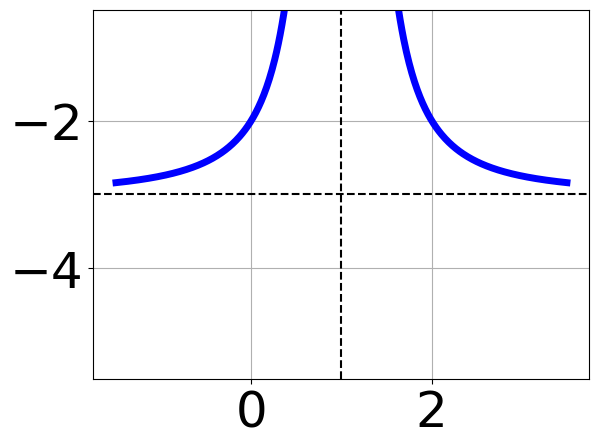
\includegraphics[width=0.5\textwidth]{../Figures/rationalGraphToEquationB.png}
\end{center}



The solution is \( \text{None of the above as it should be } f(x) = \frac{-1}{x - 1} + 1 \), which is option E.\begin{enumerate}[label=\Alph*.]
\item \( f(x) = \frac{-1}{(x + 1)^2} + 1 \)

Corresponds to thinking the graph was a shifted version of $\frac{1}{x^2}$.
\item \( f(x) = \frac{-1}{x + 1} + 1 \)

The $x$-value of the equation does not match the graph.
\item \( f(x) = \frac{1}{x - 1} + 1 \)

Corresponds to using the general form $f(x) = \frac{a}{x-h}+k$ and the opposite leading coefficient.
\item \( f(x) = \frac{1}{(x - 1)^2} + 1 \)

Corresponds to thinking the graph was a shifted version of $\frac{1}{x^2}$, using the general form $f(x) = \frac{a}{x-h}+k$, and the opposite leading coefficient.
\item \( \text{None of the above} \)

None of the equation options were the correct equation.
\end{enumerate}

\textbf{General Comment:} Remember that the general form of a basic rational equation is $ f(x) = \frac{a}{(x-h)^n} + k$, where $a$ is the leading coefficient (and in this case, we assume is either $1$ or $-1$), $n$ is the degree (in this case, either $1$ or $2$), and $(h, k)$ is the intersection of the asymptotes.
}
\litem{
Solve the rational equation below. Then, choose the interval(s) that the solution(s) belongs to.
\[ \frac{9}{-5x + 2} + -6 = \frac{3}{15x -6} \]
The solution is \( x = 0.067 \), which is option E.\begin{enumerate}[label=\Alph*.]
\item \( x_1 \in [-1.1, -0.7] \text{ and } x_2 \in [0,0.14] \)

$x = -0.733 \text{ and } x = 0.067$, which corresponds to getting the correct solution and believing there should be a second solution to the equation.
\item \( \text{All solutions lead to invalid or complex values in the equation.} \)

This corresponds to thinking $x = 0.067$ leads to dividing by zero in the original equation, which it does not.
\item \( x \in [-1.1,-0.7] \)

$x = -0.733$, which corresponds to not distributing the factor $-5x + 2$ correctly when trying to eliminate the fraction.
\item \( x_1 \in [-0.2, 0.4] \text{ and } x_2 \in [0.14,0.48] \)

$x = 0.067 \text{ and } x = 0.200$, which corresponds to getting the correct solution and believing there should be a second solution to the equation.
\item \( x \in [0.07,1.07] \)

* $x = 0.067$, which is the correct option.
\end{enumerate}

\textbf{General Comment:} Distractors are different based on the number of solutions. Remember that after solving, we need to make sure our solution does not make the original equation divide by zero!
}
\litem{
Determine the domain of the function below.
\[ f(x) = \frac{4}{15x^{2} +27 x + 12} \]
The solution is \( \text{All Real numbers except } x = -1.000 \text{ and } x = -0.800. \), which is option B.\begin{enumerate}[label=\Alph*.]
\item \( \text{All Real numbers except } x = a, \text{ where } a \in [-1.37, -0.98] \)

All Real numbers except $x = -1.000$, which corresponds to removing only 1 value from the denominator.
\item \( \text{All Real numbers except } x = a \text{ and } x = b, \text{ where } a \in [-1.37, -0.98] \text{ and } b \in [-0.84, -0.59] \)

All Real numbers except $x = -1.000$ and $x = -0.800$, which is the correct option.
\item \( \text{All Real numbers except } x = a, \text{ where } a \in [-20.28, -19.69] \)

All Real numbers except $x = -20.000$, which corresponds to removing a distractor value from the denominator.
\item \( \text{All Real numbers.} \)

This corresponds to thinking the denominator has complex roots or that rational functions have a domain of all Real numbers.
\item \( \text{All Real numbers except } x = a \text{ and } x = b, \text{ where } a \in [-20.28, -19.69] \text{ and } b \in [-9.15, -8.94] \)

All Real numbers except $x = -20.000$ and $x = -9.000$, which corresponds to not factoring the denominator correctly.
\end{enumerate}

\textbf{General Comment:} Recall that dividing by zero is not a real number. Therefore the domain is all real numbers \textbf{except} those that make the denominator 0.
}
\litem{
Solve the rational equation below. Then, choose the interval(s) that the solution(s) belongs to.
\[ \frac{4x}{-4x + 4} + \frac{-5x^{2}}{8x^{2} +4 x -12} = \frac{-6}{-2x -3} \]
The solution is \( \text{There are two solutions: } x = 0.555 \text{ and } x = -3.325 \), which is option A.\begin{enumerate}[label=\Alph*.]
\item \( x_1 \in [0.3, 1.3] \text{ and } x_2 \in [-7.33,-2.33] \)

* $x = 0.555 \text{ and } x = -3.325$, which is the correct option.
\item \( x \in [-6.5,-2.7] \)


\item \( x_1 \in [0.3, 1.3] \text{ and } x_2 \in [-2,2] \)


\item \( \text{All solutions lead to invalid or complex values in the equation.} \)


\item \( x \in [-1.8,-0.7] \)


\end{enumerate}

\textbf{General Comment:} Distractors are different based on the number of solutions. Remember that after solving, we need to make sure our solution does not make the original equation divide by zero!
}
\litem{
Choose the equation of the function graphed below.

\begin{center}
    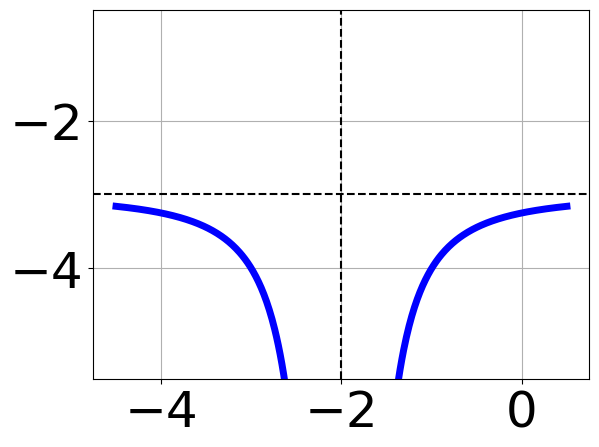
\includegraphics[width=0.5\textwidth]{../Figures/rationalGraphToEquationCopyB.png}
\end{center}



The solution is \( \text{None of the above as it should be } f(x) = \frac{1}{x - 2} - 3 \), which is option E.\begin{enumerate}[label=\Alph*.]
\item \( f(x) = \frac{1}{x + 2} - 4 \)

The $x$- and $y$-value of the equation does not match the graph.
\item \( f(x) = \frac{1}{(x + 2)^2} - 4 \)

Corresponds to thinking the graph was a shifted version of $\frac{1}{x^2}$ not noticing the $y$-value was wrong.
\item \( f(x) = \frac{-1}{(x - 2)^2} - 4 \)

Corresponds to thinking the graph was a shifted version of $\frac{1}{x^2}$, using the general form $f(x) = \frac{a}{x-h}+k$, the opposite leading coefficient, AND not noticing the $y$-value was wrong.
\item \( f(x) = \frac{-1}{x - 2} - 4 \)

Corresponds to using the general form $f(x) = \frac{a}{x-h}+k$, the opposite leading coefficient AND not noticing the $y$-value was wrong.
\item \( \text{None of the above} \)

None of the equation options were the correct equation.
\end{enumerate}

\textbf{General Comment:} Remember that the general form of a basic rational equation is $ f(x) = \frac{a}{(x-h)^n} + k$, where $a$ is the leading coefficient (and in this case, we assume is either $1$ or $-1$), $n$ is the degree (in this case, either $1$ or $2$), and $(h, k)$ is the intersection of the asymptotes.
}
\litem{
Choose the graph of the equation below.
\[ f(x) = \frac{-1}{(x + 1)^2} - 2 \]
The solution is the graph below, which is option D.
\begin{center}
    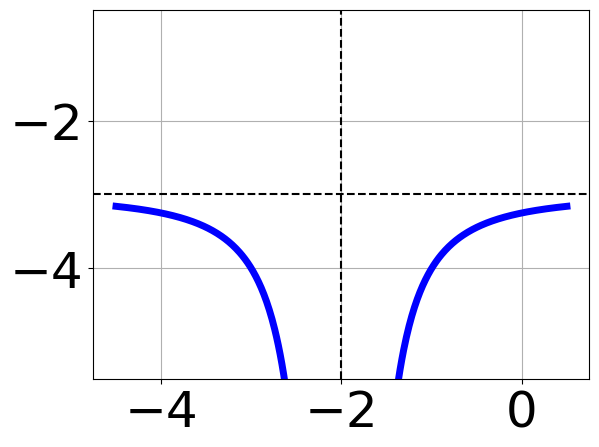
\includegraphics[width=0.3\textwidth]{../Figures/rationalEquationToGraphCopyDB.png}
\end{center}\begin{enumerate}[label=\Alph*.]
\begin{multicols}{2}
\item 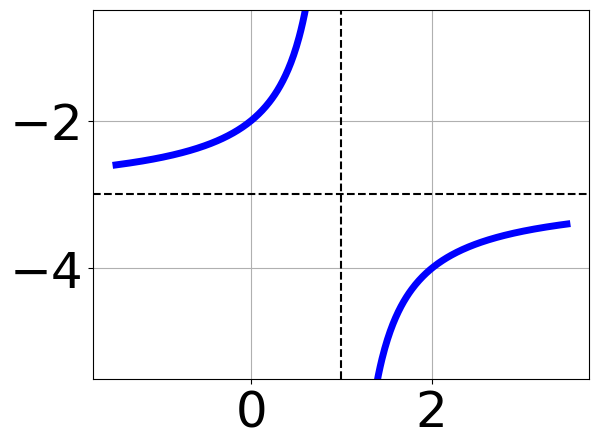
\includegraphics[width = 0.3\textwidth]{../Figures/rationalEquationToGraphCopyAB.png}
\item 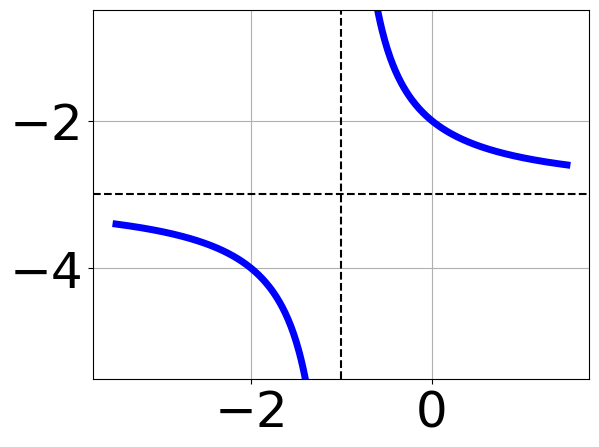
\includegraphics[width = 0.3\textwidth]{../Figures/rationalEquationToGraphCopyBB.png}
\item 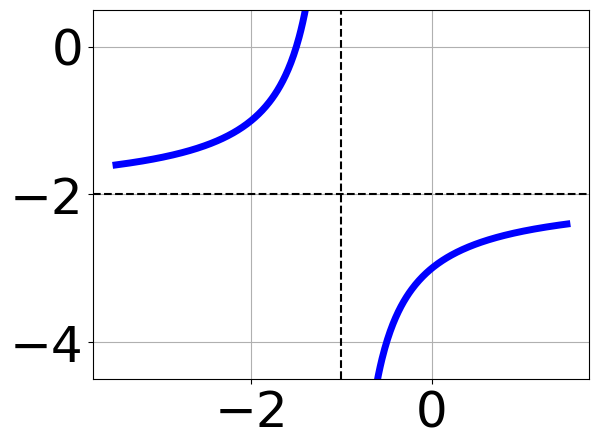
\includegraphics[width = 0.3\textwidth]{../Figures/rationalEquationToGraphCopyCB.png}
\item 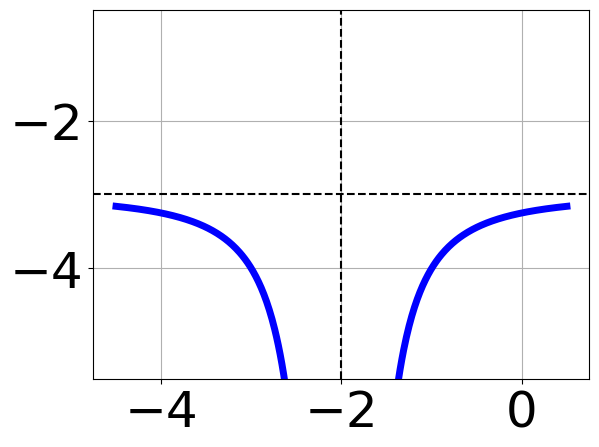
\includegraphics[width = 0.3\textwidth]{../Figures/rationalEquationToGraphCopyDB.png}
\end{multicols}\item None of the above.\end{enumerate}
\textbf{General Comment:} Remember that the general form of a basic rational equation is $ f(x) = \frac{a}{(x-h)^n} + k$, where $a$ is the leading coefficient (and in this case, we assume is either $1$ or $-1$), $n$ is the degree (in this case, either $1$ or $2$), and $(h, k)$ is the intersection of the asymptotes.
}
\litem{
Solve the rational equation below. Then, choose the interval(s) that the solution(s) belongs to.
\[ \frac{39}{117x -91} + 1 = \frac{39}{117x -91} \]
The solution is \( \text{all solutions are invalid or lead to complex values in the equation.} \), which is option E.\begin{enumerate}[label=\Alph*.]
\item \( x_1 \in [-1, 0.2] \text{ and } x_2 \in [-1.22,1.78] \)

$x = -0.778 \text{ and } x = 0.778$, which corresponds to getting the correct solution and believing there should be a second solution to the equation.
\item \( x \in [0.78,2.78] \)

$x = 0.778$, which corresponds to not checking if this value leads to dividing by 0 in the original equation and thus is not a valid solution.
\item \( x \in [-1,0.2] \)

$x = -0.778$, which corresponds to not distributing the factor $117x -91$ correctly when trying to eliminate the fraction.
\item \( x_1 \in [0.5, 1.3] \text{ and } x_2 \in [-1.22,1.78] \)

$x = 0.778 \text{ and } x = 0.778$, which corresponds to getting the correct solution and believing there should be a second solution to the equation.
\item \( \text{All solutions lead to invalid or complex values in the equation.} \)

*$x = 0.778$ leads to dividing by 0 in the original equation and thus is not a valid solution, which is the correct option.
\end{enumerate}

\textbf{General Comment:} Distractors are different based on the number of solutions. Remember that after solving, we need to make sure our solution does not make the original equation divide by zero!
}
\litem{
Solve the rational equation below. Then, choose the interval(s) that the solution(s) belongs to.
\[ \frac{3x}{-2x + 2} + \frac{-3x^{2}}{-12x^{2} +6 x + 6} = \frac{4}{6x + 3} \]
The solution is \( \text{There are two solutions: } x = 0.358 \text{ and } x = -1.491 \), which is option E.\begin{enumerate}[label=\Alph*.]
\item \( x \in [-0.62,-0.24] \)


\item \( \text{All solutions lead to invalid or complex values in the equation.} \)


\item \( x \in [-2.46,-1.41] \)


\item \( x_1 \in [-0.35, 1.15] \text{ and } x_2 \in [0.8,1.4] \)


\item \( x_1 \in [-0.35, 1.15] \text{ and } x_2 \in [-4,-1.4] \)

* $x = 0.358 \text{ and } x = -1.491$, which is the correct option.
\end{enumerate}

\textbf{General Comment:} Distractors are different based on the number of solutions. Remember that after solving, we need to make sure our solution does not make the original equation divide by zero!
}
\litem{
Determine the domain of the function below.
\[ f(x) = \frac{5}{20x^{2} +46 x + 24} \]
The solution is \( \text{All Real numbers except } x = -1.500 \text{ and } x = -0.800. \), which is option A.\begin{enumerate}[label=\Alph*.]
\item \( \text{All Real numbers except } x = a \text{ and } x = b, \text{ where } a \in [-1.75, -1.39] \text{ and } b \in [-1.03, -0.71] \)

All Real numbers except $x = -1.500$ and $x = -0.800$, which is the correct option.
\item \( \text{All Real numbers except } x = a, \text{ where } a \in [-1.75, -1.39] \)

All Real numbers except $x = -1.500$, which corresponds to removing only 1 value from the denominator.
\item \( \text{All Real numbers except } x = a \text{ and } x = b, \text{ where } a \in [-24.7, -23.67] \text{ and } b \in [-20.31, -19.93] \)

All Real numbers except $x = -24.000$ and $x = -20.000$, which corresponds to not factoring the denominator correctly.
\item \( \text{All Real numbers except } x = a, \text{ where } a \in [-24.7, -23.67] \)

All Real numbers except $x = -24.000$, which corresponds to removing a distractor value from the denominator.
\item \( \text{All Real numbers.} \)

This corresponds to thinking the denominator has complex roots or that rational functions have a domain of all Real numbers.
\end{enumerate}

\textbf{General Comment:} Recall that dividing by zero is not a real number. Therefore the domain is all real numbers \textbf{except} those that make the denominator 0.
}
\end{enumerate}

\end{document}